\chapter{Monte Carlo radiation transport technique}

\section{Introduction and Background}
This chapter will provide an overview of the Monte Carlo method and how it is used within the context of \gls{mcrt}. The chapter will then present the details of the MCRT code used as the basis of the subsequent chapters. Validation of this code and details of computational speed up are also presented. Subsequent chapters will expand upon the code for each individual projects needs.

\subsection{Monte Carlo method}
The Monte Carlo method is a numerical analysis technique based upon random numbers, which are used to calculate unknown variables in problems. 

The earliest use of the method is in Buffon's needle experiment of the 18$^{th}$ century~\cite{badger1994lazzarini,beckmann2015history,buffon1785histoire}. Buffon asked the question;

\medskip

``Suppose we have a floor made of parallel strips of wood, each the same width, and we drop a needle onto the floor. What is the probability that the needle will lie across a line between two strips?"

\medskip

The solution to this question is as:
for a needle length \textit{l}, strip separation \textit{s}, and where \textit{x} is the distance from the needle to the closest line. Then using a simple geometrical argument, a needle crosses a strip if $x \leq \tfrac{l}{2} sin \theta$.

$x$ is distributed uniformly in [0, $\tfrac{s}{2}$], and $\theta$ in [0, $\tfrac{\pi}{2}$]. Therefore the probability density function for $x$ is $p(x)=\tfrac{2}{s}$, and $\theta$ is $p(\theta) = \tfrac{2}{\pi}$. The \gls{pdf}, is a function of a variable that gives probability for a variable to a take a given value. The \gls{pdf} is normalised over the whole range of the variable, in this case $x$, and $\theta$.
Thus, as $x$ and $\theta$ are independent variables, giving a joint probability of $p(x,\theta) = \tfrac{4}{s \pi}$.
So the probability of a needle of length l ($l<s$) is:

\begin{equation}
P=\int_0^{\frac{\pi}{2}}\int_0^{\frac{l}{2}sin\theta}\frac{4}{s\pi}dx d\theta = \frac{2 l}{s \pi}\label{eqn:buffon}
\end{equation}


\Cref{eqn:buffon} can be used to carry out a Monte Carlo estimation of pi. A simple rearrangement yields: $\pi = \tfrac{2l}{sP}$ where P is the ratio of needles crossing the line over total number dropped. Laplace was the first to suggest that Buffon's needle experiment could be used to estimate $\pi$~\cite{beckmann2015history}. \Cref{fig:buffon-needle} shows an example of simulation of Buffon's needle experiment.

\begin{figure}
\centering
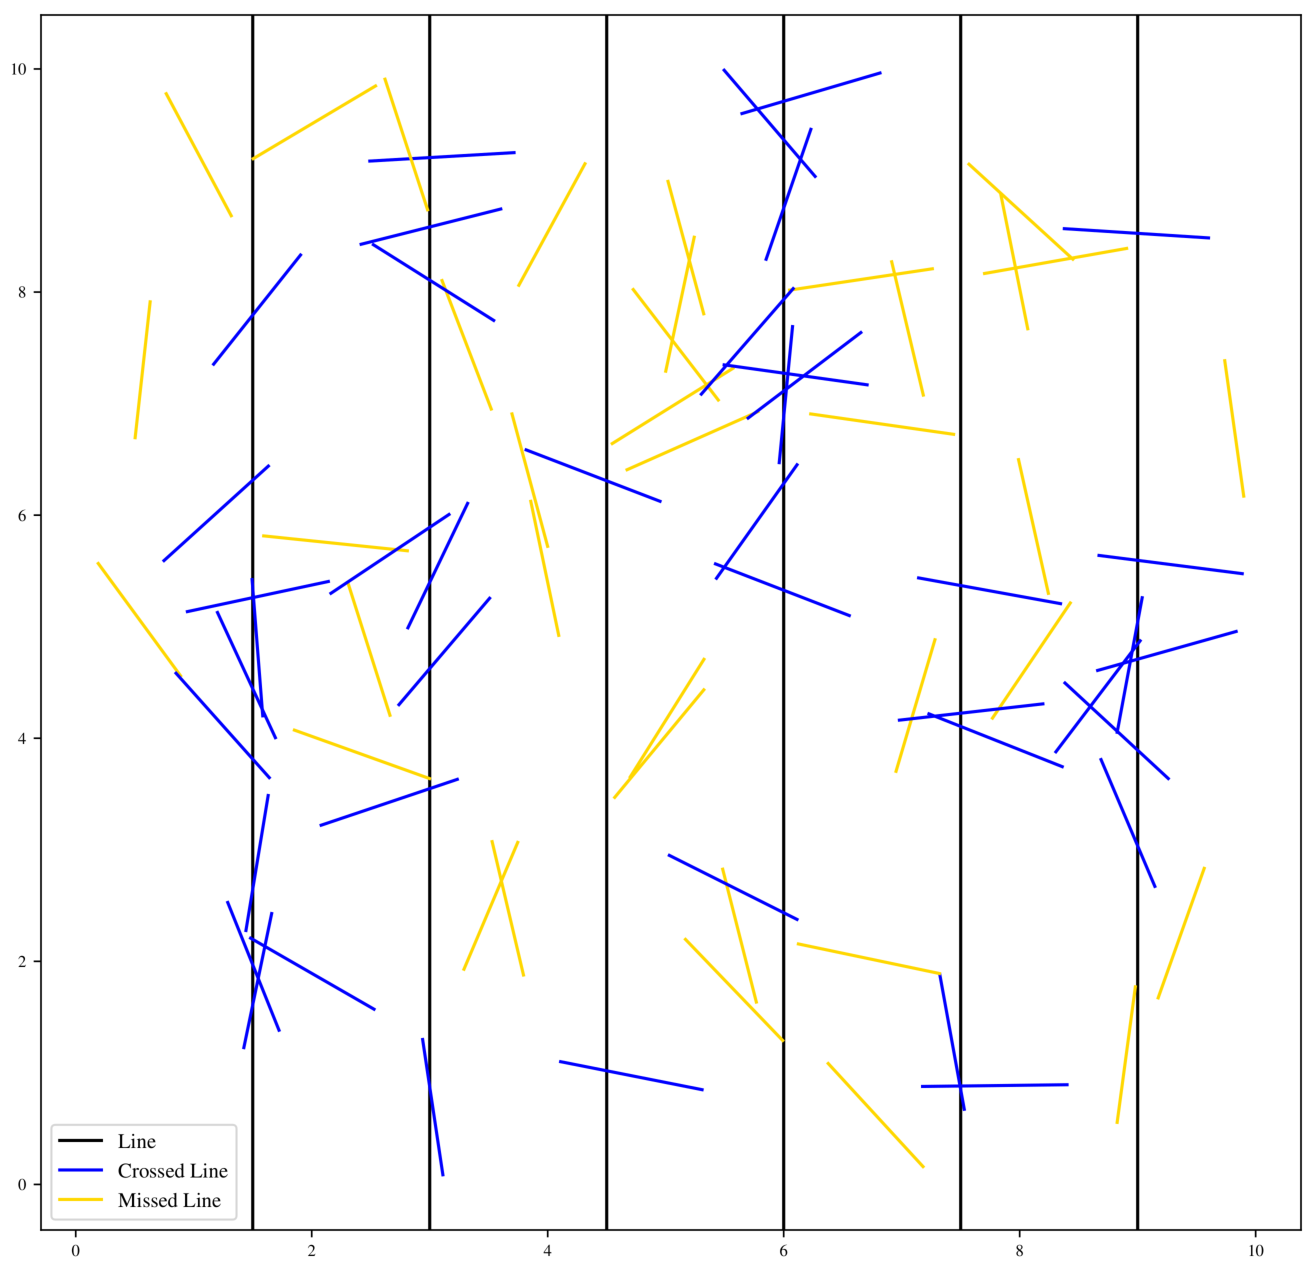
\includegraphics[width=\columnwidth/2]{./MCRT/images/buffon-pi=317.pdf}
\caption{Sample buffon needle experiment. 100 needles are dropped on a 10 by 10 cm area with lines spaced 1.5cm apart. If a needle lands on a line it is recorded and colored blue, else it is yellow. This simulation gave a value of pi as 3.17.}
\label{fig:buffon-needle}
\end{figure}

The Monte Carlo method is used in various different disciplines. Ranging from use in the financial sector to analyse investments and stocks by simulating the sources of uncertainty which affect their values~\cite{jackel2002monte,finaceprrof}, use in statistical analysis~\cite{wall2012practical}, and in modern computer generated images (see \cref{fig:ray-trace})~\cite{Kajiyarendering,Cookraytracing}.

\begin{figure}
\centering
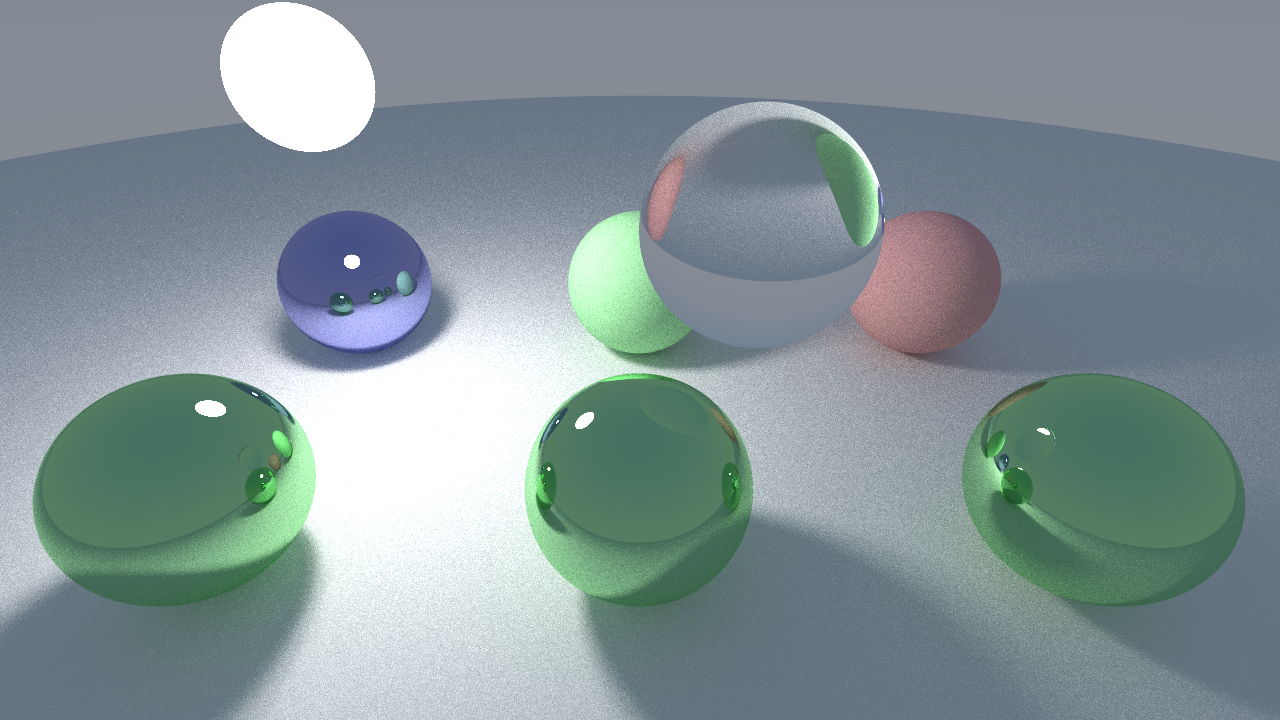
\includegraphics[width=\columnwidth]{./MCRT/images/ray-tracing.png}
\caption{Computer generated imagery using ray-tracing. Code usd to create image available at: \url{https://github.com/lewisfish/RayTran}}
\label{fig:ray-trace}
\end{figure}

\section{Monte Carlo radiation transport algorithm}

\subsection{Introduction $\&$ background}
The technique that makes up the bulk of this thesis, is the \gls{mcrt} technique. This method was developed at the tail end of World War two at the Los Alamos National Laboratory, for the purpose of calculating neutron diffusion though shielding material~\cite{montybeg1,eckhardt1987stan,anderson1986metropolis,ulam1947statistical}. It has since found a myriad of applications from light transport through dusty clouds~\cite{wood1999model}, calculating doses for radiotherapy~\cite{rogers1995beam} to light transport through tissue~\cite{1stmonty}.

\section{Validation of MCRT code}
